%----------------------------------------------------------------------------
\chapter{\AudioOverIp}
%----------------------------------------------------------------------------
\section{Bevezetés az Audio over IP világába}
%----------------------------------------------------------------------------
A 90-es évek vége óta a szakmai hangipar elmozdult a pont-pont digitális
átviteli formátumoktól (például AES/EBU vagy MADI) az IP-alapú szabványok felé
(például AES67). Ez a csomag alapú hálózati megoldás hatalmas rugalmasságot
hozott, valamint kibővített vezérlési és monitorozási képességeket biztosít
hangrendszerek számára. Lehetőséget teremt arra, hogy egy fizikailag már meglévő
telepítés későbbi szoftverkonfigurációval és frissítésekkel alkalmazkodóvá és
bővíthetővé váljon. A gyártó különböző esetekben akár teljesen új funkciókkal is
kiegészítheti a már meglévő eszközöket. 
A jelutak az IP alapú megközelítés miatt már nem kötődnek 1:1 fizikai kábelekhez, hanem
bármikor pár egérkattintással megváltoztathatóak anélkül, hogy szükség lenne bármilyen
jellegű fizikai átrendezésre, vagy dedikált audio útválasztó hardverre. 
A csomagorientált átvitel jellegéből adódik, hogy az audiojelek automatikusan eljutnak 
a kívánt helyre az IT hálózaton keresztül.
A Cirrus Logic által 1996-ban bevezetett CobraNetet
általában az első sikeres audio-over-ethernet hálózat-implementációnak tekintik,
és számos audio telepítés alapját képezi. Ezek közé tartoznak különböző kongresszusi központok,
színházak, koncerttermek, repülőterek és vidámparkok.
Bár ma is sok CobraNet telepítés létezik, magas késleltetési problémák és korlátozott mérethatékonyság
miatt nem ideális élő hang, stúdiófelvételek és rádió létesítmények számára.
A mintegy tíz évvel később megjelent egy ausztrál cég az Audinate, és az általuk kifejlesztett
Dante a `Digital Audio Network Through Ethernet'. Dante több jelentős
előnnyel rendelkezik az első generációs audio-over-IP technológiákhoz viszonyítva.
Ezek közé értve a jobb használhatóságot és magasabb kompatibilitást a szabványos
hálózati infrastruktúrával. A Dante egy hatalmas hardveres ökoszisztémából
profitál, több száz gyártó által gyártott ezernél is több eszközzel. 
Mielőtt a Dante elérte volna jelenlegi domináns pozícióját, nagy várakozás volt egy AVB
(Audio Video Bridging) nevű technológia körül.
Más iparágak, például az autóipar és az ipari automatizálás, átvették az AVB-t, és
általánosabb nevet adtak neki, mivel az már nem csak hang és videóalkalmazásokhoz kapcsolódik.
Az AVB-t a gyártók fejlesztőcsoportja, az AVnu Alliance időérzékeny hálózat (TSN) néven nevezte el.
Később a Milan munkacsoport, egy audio/video gyártókból álló konzorcium, úgy
döntött, hogy kidolgoz egy finomhangolt specifikációt a profi audio/video
rendszerekben való használatra, Milan néven. 
Ez egy specifikus TSN verzió, amely az audio/video szolgáltatók közötti interoperabilitásra összpontosít.
Ez nem a TSN alapján történt, mivel a TSN-hez speciális IT hardver szükséges az audio
követelmények kezeléséhez, és csak korlátozott számú kapcsolómodell támogatja a TSN-t. 
%----------------------------------------------------------------------------
Az átmenet az IP hálózatokra összehasonlítható az analóg hangról a digitális
hangra való átmenettel. Először csak néhány kezdeti telepítés, amelyek az új technológiát
használják, majd esetleg hiányosságokat mutathatnak a kezelés vagy a megbízhatóság
terén a hagyományos régi megközelítéshez képest, de ezek idővel a technológia fejlődésével eltűnnek. 
Vannak területek, ahol az IT hálózatok alapvetően más módon működnek, mint a hagyományos audio útválasztás.
Először is, egy szabványos IT hálózat nincs kialakítva szigorú időzítési követelmények
teljesítésére, amelyek általában az audio esetében jellemzőek. 
Egy hálózati környezetben az adatcsomagok útját más csomagok is akadályozhatják, ami jelentős
időbeli változást eredményezhet az érkezési időben.
A hagyományos audio kábelek esetében az adatok továbbításának időzítése nem változott meg a kábel által.
Másodszor, egy csomag elvesztése elfogadhatónak tűnhet és tűnik a szokásos IT
alkalmazások esetében, mivel azok automatikusan újraküldésre kerülnek, ha elvesznek.
Az audio alkalmazások esetében a késleltetés minimalizálása érdekében
létfontosságú, hogy a csomagok az első alkalommal a korrekt helyre érkezzenek meg, mivel egyáltalán nincs
elegendő idő az újraküldéshez. Ha néhány csomag elveszik, az azonnal hallható megszakításokat és kimaradásokat okoz.
A csomagvesztés gyakori oka a linkek túlterhelése, vagy a túl alacsony pufferméret.
Az audiohálózatokat oly módon kell kialakítani, hogy elegendő sávszélesség álljon rendelkezésre
minden felhasználójuk számára. Ha ez teljesül, és a csomagkiszállítás időben történik, ahogyan az audio alkalmazások igénylik,
akkor a hálózatunk már elméletileg képes stabilan működni.
Érdemes túlbiztosítani a hálózatot oly mértékben, hogy minden csomag időben
megérkezzen, anélkül, hogy további finomításra lenne szükség a kapcsolók
konfigurációjában. Konkrétan ez azt jelenti, hogy olyan IT hálózatokat kell
építeni elegendő sávszélességgel, és kizárólag az audio alkalmazások számára
kell használni, tehát ne keveredjenek általános mindennapi alkalmazásokkal. 
%----------------------------------------------------------------------------
A legtöbb audio-over-IP technológia abból indul ki, hogy az alapul szolgáló
hálózat megfelelően fog működni. Gondolva itt arra, hogy nincsen csomagvesztés, 
nincs súlyos ütközés más csomagokkal a kapcsoló hardveren. 
Néhány hálózatban, különösen ha az audio és más forgalmat keverik, 
fontos lehet az audio és szinkronizációs csomagoknak elsőbbséget biztosítani másokkal szemben,
például az internetes böngészéssel szemben. Ez a mai legtöbb kereskedelmi forgalmazott
kapcsolóval elérhető. 
Példa audio over IP hálózatokra:
%----------------------------------------------------------------------------
\begin{itemize}
	\item Audinate által kifejlesztett Dante
\end{itemize}
\begin{itemize}
	\item QSC által kifejlesztett Q-LAN
\end{itemize}
\begin{itemize}
	\item Lawo és Partnerei által kifejlesztett RAVENNA
\end{itemize}
%----------------------------------------------------------------------------
\begin{figure}[H]
	\centering
	
\includegraphics[width=60mm, keepaspectratio]{figures/dante_logo.jpg}
	\caption{Audinate Dante logó}
	\label {fig:dante_logo}
\end{figure}
%----------------------------------------------------------------------------
\subsection{Előnyök és hátrányok}
%----------------------------------------------------------------------------
Az IT hálózatok alkalmazása hangkapcsolatokra nézve számos előnyt kínál:
\begin{itemize}
	\item Rugalmasság a hangkapcsolatok hozzáadásához vagy módosításához anélkül,
	      hogy a kábeleket cserélnénk.
\end{itemize}
\begin{itemize}
	\item Az IT viszonylag alacsony áron széles skálájú funkciót kínál.
\end{itemize}
\begin{itemize}
	\item Az alkalmazkodás és integráció az IT hálózati infrastruktúrába
	      specifikus audio vagy videokábelek alkalmazása nélkül.
\end{itemize}
\begin{itemize}
	\item Videójel és vezérlési adatok továbbíthatók ugyanazon infrastruktúrán
	      keresztül.
\end{itemize}
%----------------------------------------------------------------------------
Ugyanakkor az audio-over-IP hálózatok felhasználóit számos kihívás elé is állíthatják:
%----------------------------------------------------------------------------
\begin{itemize}
	\item Azért mert általában több hangmintát egy csatornából egy csomagba helyeznek
	      el a hatékonyság érdekében, adott minimális késleltetés adódik, mivel az
	      küldőnek meg kell várnia, hogy a hangminták rendelkezésre álljanak, mielőtt
	      azokat átküldené a hálózaton. Ez a késleltetés általában magasabb, mint a
	      pont-pont digitális hangszabványok esetében, de optimalizált csomagformátumok és
	      hálózati beállítások segítségével minimalizálható és nagyon jól közelíthető.
\end{itemize}
\begin{itemize}
	\item Mivel az IT hálózatok nem meghatározottak a csomagok úti idejét tekintve,
	      egy biztonsági tartományt, azaz egy audio buffer-t kell beszúrni a fogadó végén.
	      Ez a buffer további késleltetést eredményez. Minél kevesebb csomagütközés van
	      jelen a hálózatban, annál inkább csökkenthető ez a biztonsági tartomány (és
	      ezzel a késleltetés).
\end{itemize}
\begin{itemize}
	\item Az audio csomagformátumok változatossága miatt növekszik a komplexitás,
	      ami azt jelenti, hogy a fogadóknak és küldőknek azonos beállításokkal kell
	      rendelkezniük. Az audio-over-IP technológia komplexitása jelentősen magasabb,
	      mint az előző technológiáké. Az iparág még mindig jelentős munkát végez annak
	      érdekében, hogy csökkentse ezt a komplexitást a felhasználó számára, bevezetve
	      intelligens és felhasználóbarát szoftvermegoldásokat az audiohálózatok
	      kezelésére.
\end{itemize}
%----------------------------------------------------------------------------
\subsection{Fázishelyesség}
%----------------------------------------------------------------------------
A legtöbb audio alkalmazásban kritikus a több eszköz szinkronizált viselkedése.
Elengedhetetlen a mikrofonok vagy hangszórók közötti fázispontosság.
Amikor több hangszóró van csatlakoztatva egy erősítőhöz, és az összes csatorna
egyetlen hangcsomagban érkezik meg, nincs veszélye annak, hogy a csatornák
ellenfázisban lennének egymással, mivel a hangminták nem változhatnak el egymás
között a hálózaton keresztüli átvitel során. 
Azonban egyre több alkalmazásban több erősítő és processzor függetlenül kap hangcsomagokat,
miközben továbbra is szükség van arra, hogy pontosan reprodukálják az audiojeleket egyező fázispontossággal.
Ezért egy adott audio csomagot több hálózati eszköz is megkaphatja, pufferelheti, és ezeket
pontosan ugyanabban az időben kell lejátszania. 
Mivel nincsenek szoros időzítési specifikációk az IT hálózatokban a csomagok továbbításának és
megérkezésének időpontjára vonatkozóan, az audiohálózatoknak mindenképpen szinkronizációs
módszert kell biztosítaniuk. Ez egy fontos, de új probléma a hálózatokban, amellyel az összes
audio-over-IP technológiának foglalkoznia kell.
Az audiohálózaton belül minden eszköz abszolút időben szinkronizált
a Precision Time Protocol (PTP) szerint. Ez azt jelenti, hogy belső óráik (PTP
követők) egy referenciaóra eszközből (PTP vezető) származnak. Ez az eszköz
bármilyen audioeszköz lehet, amely biztosítja ezt a funkciót, vagy akár egy
speciálisan erre a célra kifejlesztett termék is lehet a pontos PTP órák előállítására.
A vezetőt egy felhasználói beállítás vagy alternatívaként egy szabványos
automatizmus választja ki. Az összes eszköz számára, legyen az audio adó vagy
vevő, az a végső követelmény, hogy pontosan szinkronizálódjanak ehhez az adott időhöz.
Az audio csomag küldési pillanatában egy időbélyegzővel látják el. A felhasználó állandó időeltolást állít be az
összes vevőnél, ez a linkeltolás. Amikor egy csomag megérkezik egy vevőhöz, a
pufferben marad, amíg lejátszásra kerül. Tehát az audio lejátszás pillanata a
küldési idő plusz a linkeltolás. Minden vevő két feltétel mellett érheti el egymás
között a fázispontosságot: 
Pontos időszinkronizálás a PTP óra vezetőjéhez (azonos időbázis) 
Azonos linkeltolási érték beállítása a felhasználó által az összes vevőeszközön
Ezért a linkeltolást az érintett összes kapcsolat legrosszabb esetű késleltetése alapján kell kiválasztani. 
Javasolt bizonyos engedményt hozzáadni az esetleges csomagkiszállítási idők váratlan eltéréseinek esetére,
ez azt jelenti, hogy kicsivel nagyobb időt hagyunk az átlagos csomagfeldolgozási időnél.
Szerencsére ez a koncepció elterjedt és jelenleg minden audiohálózati szabványban és a videóban is használatos. 
%----------------------------------------------------------------------------
\begin{figure}[H]
	\centering
	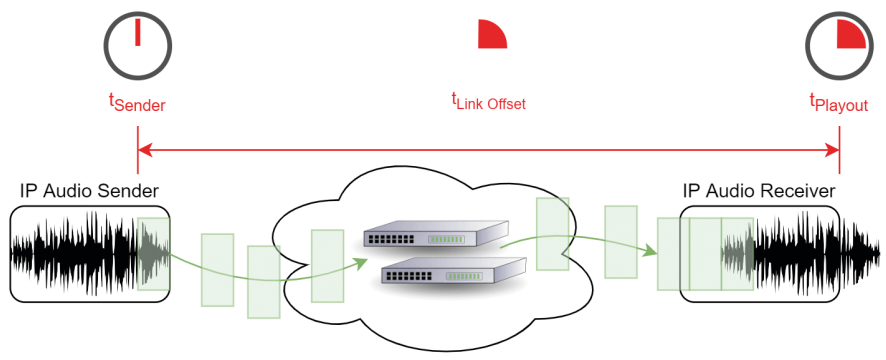
\includegraphics[width=\linewidth, keepaspectratio]{figures/link_offset_latency.png}
	\caption{A kapcsolati eltolás meghatározza a késleltetést \cite{AHNERT2023}}
	\label {fig:link_offset_latency}
\end{figure}
%----------------------------------------------------------------------------
\begin{figure}[H]
	\centering
	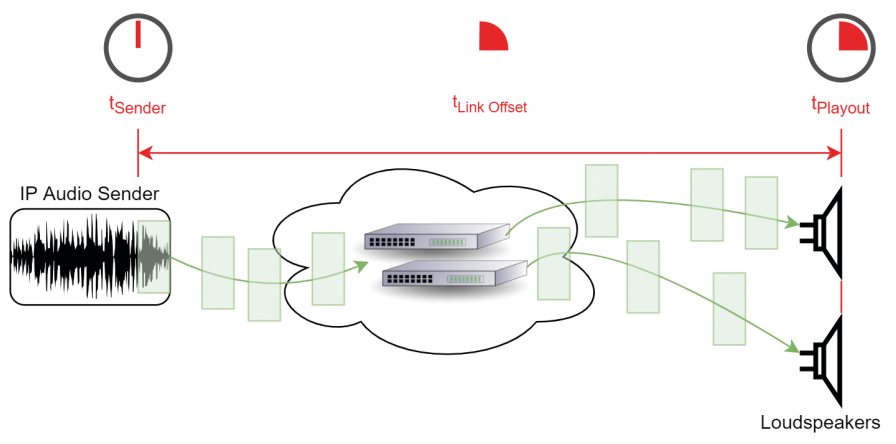
\includegraphics[width=\linewidth, keepaspectratio]{figures/phase_coherence_link_offset.png}
	\caption{Fáziskoherencia azonos kapcsolati eltolással \cite{AHNERT2023}}
	\label {fig:phase_coherence_link_offset}
\end{figure}
%----------------------------------------------------------------------------
\subsection{Szinkronizáció}
%----------------------------------------------------------------------------
Az IP küldők és fogadók szinkronizációja az alacsony késleltetéssel való szinkronban lévő működéshez elengedhetetlen.
A hagyományos audio technológiákban az eszközöket vagy külön \textit{word clock} kapcsolattal, 
vagy szinkronizált audio formátumokkal, például AES/EBU vagy MADI segítségével szinkronizálták.
A fogadók közvetlenül képesek voltak azokból az formátumokból frekvenciájukat és fázisukat kinyerni,
mivel valamiféle \textit{impulzust} biztosítottak, ami jelzi a pillanatot, amikor egy
audio minta létrejön vagy lejátszódik, például analóg-digitális konverterek esetében.
Az PTP csomagok kicsik és nem tartják fel a forgalmat sokáig, de fontos, hogy a
kapcsolókban a lehető legmagasabb prioritással továbbítsák őket. 
Ez végül növelni fogja a szinkronizáció pontosságát. 
A QoS-hez (Quality of service) kapcsolódóan ez azt jelenti, hogy a PTP csomagokat még a hangnál is magasabb prioritással kell
kezelni. Az összes hálózati eszközt ugyanazon naptári időpontra szinkronizálják a Precision Time Protocol
(PTP) segítségével. Ennek az időnek a kiindulása egy olyan eszköz, amelyet óraleadernek
neveznek, míg az ehhez igazodó eszközöket óra követőknek hívják. 
Minden eszköznek meg kell hozzá generálnia a kívánt hagyományos órát (például 96 kHz), amelyet a PTP-n keresztül kapott
abszolút időből származtat. Ez a belső óra a \textit{médiaóra}. 
Ha a gyártó megfelelően implementálja, minden eszköz médiaórájának pontosan ugyan annyinak kell lennie a
frekvencia és fázis terén. A magas pontosság technikailag elérhető, de kihívást
jelent az audio gyártók számára. Ezért a PTP szinkronizált eszközök közötti
fázispontosság minőségtől függően változhat. Elfogadható változásnak tekinthető ha az kisebb mint <1 µs, azaz 1 mikroszekundum.
%----------------------------------------------------------------------------
Mivel az IT hálózatok nem eléggé determinisztikusak a csomag kézbesítésének időpontját
illetően, a készülékek pontos szinkronizációja kifinomult megközelítést igényel.
A PTP követők fő feladata két hatás kompenzálása, amelyek bármilyen hálózat esetén előfordulhatnak:
%----------------------------------------------------------------------------
\subsubsection{Jitter kompenzáció}
%----------------------------------------------------------------------------
A PTP vezető által a szinkronizációs üzenetekben megadott jelenlegi időt az összes követőnek egy jól ismert multicast
cím (224.0.1.129) használatával mutatják be. 
A hálózat és a kapcsolók sorai természetükből adódóan ez az információ nem mindig érkezik meg állandó
késleltetéssel a vevő számára. 
Ez a változás a csomag jitter vagy csomag késleltetési változás (PDV) néven ismert effektus,
ezt az elváltozást minden PTP követőnek kompenzálnia kell. 
Általában az audio hálózatok 1--8 üzenet/mp szinkronizálási arányt
használnak. (A 8-as maximális érték csak kompatibilitás érdekében javasolt)
%----------------------------------------------------------------------------
\subsubsection{Késleltetés mérése}
%----------------------------------------------------------------------------
A követő második kulcsfontosságú feladat a vezető és a követő közötti
csomagkésleltetés mérése a vezető által a szinkronizációs üzenetekben kapott
idő kijavításához. Ehhez szükség van arra az időmérésre, amelyek azt mutatja meg számunkra,
hogy a hálózati út során mennyi időbe telik egy csomag átvitele.
Ez a mérés magában foglalja az összes közöttük lévő
összetevő késleltetését, beleértve a kábeleket és kapcsolókat is. 
A vezető és a követő közötti kábelhossz és a kapcsolók száma nem számít, csak a végső érték.
A PTP időnek az összes követő között ugyanannak kell lennie nanoszekundum pontossággal.
Az egyetlen feltétel a PTP számára, hogy a késleltetés mindkét irányban, a vezetőtől a
követőig és fordítva, állandó és szimmetrikus maradjon.
A késleltetést a követő két üzenet cseréjével méri, a késleltetési kérésből és a késleltetési válaszból következően.
Ezt a késleltetést általában a szinkronizálási aránnyal azonos gyakorisággal hajtják végre, 
azaz az előbbiekben már említett 1 és 8 alkalom között.
Mivel egy vezetőnek minden egyes követővel üzenetet kell cserélnie, van egy maximális követőszámra
vonatkozó korlátja. Sajnálatos módon ez nincs egyértelműen meghatározva, mivel
ez az érték a használt üzenetsebességektől függ.
%----------------------------------------------------------------------------
Mivel a hálózaton több eszköz is képes lehet PTP vezetőként működni és elosztani
az időt az összes követőnek, a szabvány szabályokat hozott létre a vezető
kiválasztásához. Ezt a szabályt a Best Master Clock Algorithm (BMCA), vagyis a
Legjobb Mesteróra Algoritmusnak nevezik. Minden vezetőképes eszköz küldhet
bejelentő üzeneteket a prioritásairól (amelyeket a felhasználó állít be),
valamint az oszcillátor pontosságáról. Ezenkívül figyelnie kell más eszközöket,
amelyek szintén elküldhetik saját bejelentő üzeneteiket. 
Ha más bejövő üzenetek jobb minőséget jelentenek, az eszköz leállítja a vezetőként való bejelentkezését.
Ellenkező esetben rendszeresen küldi saját üzeneteit, mintegy \textit{szívverésként},
és ezzel jelezve minden másik eszköznek az aktív állapotát. 
Ezeket az üzeneteket az announce intervallumnak nevezett időközönként küldik el. 
A bejelentő üzenetek szolgálnak \textit{szívverésként} is, hogy mások tudják, a jelenlegi mester még működőképes.
Ha a kapcsolat megszakad, az összes egység vár egy bizonyos időt (bejelentő időtúllépés),
amíg elküldik bejelentő üzeneteiket, majd megismétlik a kiválasztási folyamatot. 
A vezetőváltás idején a követőknek folytatniuk kell saját oszcillátoruk belső működését.
Az audio nem szakítható meg a vezetőváltás során.
A bejelentő üzenetekben megadott minőség két értéket tartalmaz, amelyeket a felhasználó állít be: prioritás 1 és prioritás 2.
Mindkettő értéke 0 és 255 között változhat, ahol az 0 a legjobb és legyőzi a többieket.
Ha egy prioritás 1 érték kisebb egy eszközön, mint más eszközökön,
akkor az lesz a vezető. A prioritás 2 alatti érték csak akkor releváns, ha
minden előző érték, beleértve a prioritás 1-et is, több eszközön ugyanaz. 
Ez előfordulhat két azonos típusú eszköz telepítéseknél, amelyeknek a felhasználó
azonos értéket állított be a prioritás 1-hez. Ebben az esetben a prioritás 2
határozza meg, hogy melyik lesz a fő vezető, és melyik a tartalék. 
Fontos megjegyezni, hogy néhány eszköz nem kínál lehetőséget a felhasználónak ezen értékének megadására.
Ehelyett egyszerűen a \textit{Preferált Vezető} megjelölésével rendelkeznek.
Technikailag ezek a termékek rögzített értéket használnak bejelentő üzeneteikben, amit a gyártó határoz meg.
Ezért még mindig lehetséges, hogy egy másik PTP vezetőnél beírva egy még alacsonyabb értéket, felül bírálhatja az ilyen típusú eszközt.
Néhány eszköz támogatja azt a beállítást is, amit \textit{Csak Követő} néven ismerünk. Ebben az esetben amikor ez engedélyezve van,
az adott eszköz sosem próbálja meg átvenni a vezetői szerepet az PTP hálózaton.
%----------------------------------------------------------------------------
\subsection{Mintavételi frekvencia és bitmélység}
%----------------------------------------------------------------------------
Az audio over IP rendszereknél a kifogástalan működéshez elengedhetetlen a számunkra
megfelelő mintavételi frekvencia és bitmélység meghatározása.

Ezek a paraméterek alapvetően befolyásolják az audio minőségét és a hálózati teljesítményt.
Fontos figyelembe venni az átviteli kapacitást, valamint az egyes eszközök maximális mintavételi frekvenciáját és bitmélységét.
Amennyiben a hálózat nem képes a megfelelő sávszélesség biztosítására, a hálózatunk instabillá válhat, 
hangkimaradások és megszakadások, legrosszabb esetben a hálózat összeomlása is előfordulhat.
A gyakran alkalmazott 48 kHz-es mintavételi frekvencia széles hangsávot biztosít, és kompatibilis a legtöbb
professzionális hangtechnikai alkalmazással. 
Nemrégiben kezdett el jobban elterjedni szélesebb körben is a 96 kHz-es mintavételi frekvencia, ami
nagyobb részletességet és jobb hangminőséget eredményez, de cserébe nagyobb sávszélességet igényel.
A sávszélesség kiszámítása a következő képlettel történik:
%----------------------------------------------------------------------------
\begin{equation}
	\label{eq:sávszélesség}
	Sávszélesség igény = MintavételiFrekvencia * BitMélység * CsatornákSzáma
\end{equation}
%----------------------------------------------------------------------------
Ezzel a formulával könnyen és gyorsan kiszámíthatjuk, hogy a rendszerünknek mekkora sávszélességre lesz szüksége.
Tehát ha egy 64x64 csatornás rendszerünk van, 96 kHz-es mintavételi frekvenciával és 24 bites bitmélységgel,
akkor a sávszélességünk a következő lesz:
%----------------------------------------------------------------------------
\begin{equation}
	\label{eq:sávszélesség}
	96000 * 24 * 64 * 2 = 294912000 bit/s = 294,912 Mbit/s (nyers adatfolyam)
\end{equation}
%----------------------------------------------------------------------------
Mivel a hálózatunkat a Dante által ajánlott méretezés szerint szeretnénk kialakítani,
legalább 30 százalékos túlméretezést kell alkalmaznunk. Tehát a fenti példában a sávszélességünk a következő lesz:
%----------------------------------------------------------------------------
\begin{equation}
	\label{eq:teljes-sávszélesség}
	294912000 bit/s * 1.3 = 383385600 bit/s = 383,3856 Mbit/s (teljes sávszélesség)
\end{equation}
%----------------------------------------------------------------------------
A számítások alapján egy átlagos 1 Gbit/s (1 Gbit/s = 1000 Mbit/s) sávszélességű hálózaton ez a rendszer már megfelelően működhet.
Érdemes a hálózatunkat túlbiztosítani, hogy a rendszerünk a legnagyobb terhelés alatt is megfelelően működjön.
A bitmélység a hangsáv digitális reprezentációját határozza meg, és az adatok pontosságát befolyásolja.
Általában 16 vagy 24 bitmélységű rendszerek használatosak az audio over IP területén, de a Dante rendszerek a 
32 bites bitmélységet is támogatják. A 16 bites reprezentáció megfelelő lehet olyan alkalmazásokhoz, ahol a nagy
dinamikatartomány nem kritikus. Ugyanakkor a 24 bites felbontás lehetőséget nyújt a pontosabb és részletesebb hangátvitelhez,
általában zenei stúdiókban és élőzenei környezetekben. 
A 32 bites bitmélység a legmagasabb minőséget biztosítja, de a sokkal nagyobb sávszélesség igénye miatt elsősorban csak
a kiemelten professzionális stúdiókban használják.
%----------------------------------------------------------------------------
\subsection{Késleltetés}
%----------------------------------------------------------------------------
Amennyiben egy csomag például 1 ms (milliszekundum) hanganyagot tartalmaz, a kapcsolat
késleltetése mindig nagyobb lesz, mint 1 ms.
A küldőnek először 1 ms hangot kell pufferelnie, mielőtt beleteszi egy csomagba, majd elküldi a hálózaton.
Ezt követi a hálózaton történő utazás ideje az összes kapcsolóval, mielőtt végül eljutna a fogadó eszköz pufferébe.
%----------------------------------------------------------------------------
\begin{enumerate}
    \item Csomag idő
    \item Utazási idő a hálózaton
    \item Fogadási puffer
\end{enumerate}
%----------------------------------------------------------------------------
A gyakorlatban a link offset technikai kifejezés egyenlő a késleltetés fogalmával.
A felhasználó felelőssége, hogy olyan link offsetet válasszon, amely elég hosszú, hogy a fogadó puffer soha ne ürüljön ki, és
ezáltal soha ne történjen meg a hang megszakítása. 
%----------------------------------------------------------------------------
\subsection{IP címek és maszkok}
%----------------------------------------------------------------------------
Egy hálózaton belül minden eszköznek egyedi címre van szüksége annak érdekében,
hogy a csomagok sikeresen elérjék a céljukat és elkerüljük a csomagok ütközését.
Egy ilyen cím lehet hardverrel kapcsolatos (MAC-cím) vagy konfigurálható a cím (IP-cím).
%----------------------------------------------------------------------------
\section{IP-cím hozzárendelési módszerek}
%----------------------------------------------------------------------------
Az IP-címeket háromféleképpen lehet hozzárendelni egy eszközhöz:
%----------------------------------------------------------------------------
\begin{itemize}
    \item \textbf{Felhasználói kézi beállítás:}
    Ez dokumentációt és felhasználói fegyelmet igényel annak érdekében,
	hogy egy adott IP-címet csak egyszer használjanak ugyanabban a hálózatban.
	Ez lehet a preferált megközelítés állandó telepítések esetén,
	mivel lehetővé teszi az IP-címek rendelésének bizonyos struktúrájának követését.
    
    \item \textbf{DHCP szerver általi eszközhöz rendelés:}
    Ez egy rugalmas, mégis strukturált módja az IP-címek elosztásának a hálózaton belül.
	Egy hoszt 'DHCP módban' megpróbálja megtalálni a megfelelő DHCP szerveret,
	és minden szükséges IP-konfigurációt egy jól szabványosított módon szerez be.
	Egy felhasználó ellenőrizheti a DHCP szerverben észlelt eszközöket és azok IP-címeit.
	Az adminisztrátor konfigurálhatja úgy, hogy csak bizonyos IP-cím-tartományt osztanak ki,
	míg másokat kézi rendelésre tartalékolnak.
    
    \item \textbf{Hoszt általi önkiosztással:}
    Ez a mechanizmus még \textit{Zeroconfig} néven ismert, és csak kis telepítésnél
	működik a korlátai miatt, mivel az összes eszköz egy alhálózatban van,
	és nem csatlakozhat más alhálózatokhoz.
\end{itemize}
%----------------------------------------------------------------------------
Egy adott eszköz IP-címéről való információ beszerzése alapvetően kissé nehéz lehet,
ha az nem jelenik meg egy kijelzőn. 
Szoftveres eszközök elérhetők az eszközök jelenlétének szkennelésére IP-cím-tartományokban,
de az IT osztályok gyakran tiltják az ilyen eszközök használatát.


Azonosítani, hogy két IP-cím ugyanabba az alhálózatba tartozik-e, nem lehetséges 
a hozzájuk tartozó alhálózati maszkok ellenőrzése nélkül.
Ha egy csomag cél-IP-címe nem ugyanabban az alhálózatban van,
a küldő eszköznek a router IP-címére kell irányítania, ahelyett hogy
közvetlenül a fogadó eszközhöz küldené. 
Két hoszt ugyanabban az alhálózaton belül hasonló IP-címekkel rendelkezik, csak az utolsó számjegyekben
különbözik. Az első részt hálózati címkének nevezik, a másodikat, amely az
eszköz számára egyedi, hosztcímkének. A kettő közötti szétválasztást az
alhálózati maszkban a `0'-s számjegyek pozíciója jelzi.
A hálózati címkét az alhálózati maszkban egy `0'-nál nagyobb érték jelzi,
míg a hosztcím a maradék jobb oldal, ahol az alhálózati maszk `0'-át jelzi.
%----------------------------------------------------------------------------
\begin{figure}[H]
    \centering
    \begin{minipage}{0.45\textwidth}
        \centering
        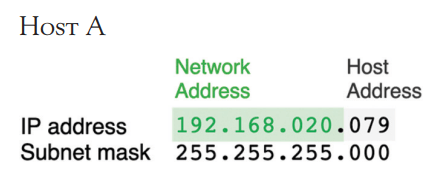
\includegraphics[width=67mm, keepaspectratio]{figures/host_a.png}
        \caption{Host A}
    \end{minipage}\hfill
    \begin{minipage}{0.45\textwidth}
        \centering
        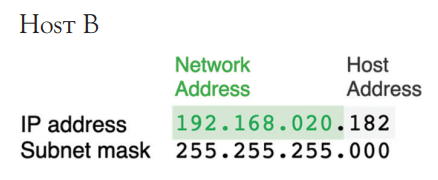
\includegraphics[width=67mm, keepaspectratio]{figures/host_b.png}
        \caption{Host B}
    \end{minipage}
\end{figure}
%----------------------------------------------------------------------------
Host A Host B  Host B ugyanabban az alhálózatban van,
mint Host A, mert mindkettő ugyanazt a hálózati címkét használja (192.168.020).
Az IP-cím hálózati része az a rész, ahol az alhálózati maszk 255-ös értéket
mutat. Ezen két eszköz között egy router nem szükséges. 
%----------------------------------------------------------------------------
\begin{figure}[H]
	\centering
	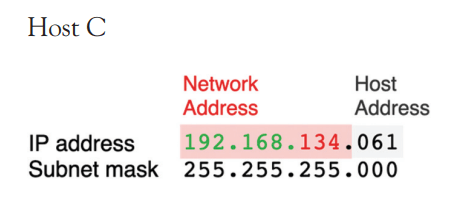
\includegraphics[width=67mm, keepaspectratio]{figures/host_c.png}
	\caption{Host C}
	\label {fig:host_c}
\end{figure}
%----------------------------------------------------------------------------
Host C más alhálózatban van, mint Host A és B, mert különbözik a hálózati címében (192.168.134, nem pedig 192.168.020).
Host C nem tud csomagokat cserélni A és B eszközökkel egy router nélkül. 
Annak érdekében, hogy ez az eszköz kommunikálhasson A és B-vel, más IP-címet kell kapnia,
kezdve a 192.168.134\ldots címmel. 
Vagy más alhálózati maszk is választható az egész beállításhoz,
például 255.255.0.0.
%----------------------------------------------------------------------------
A feljegyzett alhálózati maszkok decimális jelölése dot-decimális jelölésnek nevezik.
Azért, hogy az információt rövidebben jelezzék, gyakran
használt alternatív módszer a CIDR vagy perjeljelölés.
Az IP-cím után azonnal következő perjel után az




alhálózati maszkot a `0'-nál nagyobb értékeket mutatva jelöli meg.
Ez a jelölés az alhálózati maszk bináris formájára utal, tehát a `255' a `11111111' -nek felel meg.
A fenti példákban az alhálózati maszkok tehát bináris formájukban 24
`1'-t tartalmaznak. 
A fenti példában szereplő hosztok CIDR jelölése:
%----------------------------------------------------------------------------
\begin{itemize}
    \item \textbf{Host A:} 192.168.020.182/24
    \item \textbf{Host B:} 192.168.020.079/24
    \item \textbf{Host C:} 192.168.134.61/24
\end{itemize}
%----------------------------------------------------------------------------

A routereket használó és több alhálózatot összekapcsoló telepítések a
az OSI modell 3. rétegén működnek. Ez a modell hét rétegre osztja a
hálózatok általános funkcionalitását, mindegyik egy adott készletet ír le a hálózati
eszközök által nyújtott funkcionalitásokról. Gondolva itt elsősorban a csomagok továbbításáról a
megfelelő címzett felé. Az összes jelenlegi IT eszköz követi ezt a jól
meghatározott absztrakciós rétegkoncepciót, hogy elősegítse a gyártók közötti
interoperabilitást. A 3. rétegen működő telepítések értelmezhetik az IP-címeket,
az alhálózati maszkokat stb., és így továbbítani tudják a csomagokat az
alhálózatok között. Az itt tárgyalt összes technológia képes ilyen
forgatókönyvekben működni. Ezzel szemben néhány technológia korlátozott a 2.
rétegre. Ez azt jelenti, hogy a csomagjaikat kizárólag MAC-címek alapján
szállítják, és nem tartalmaznak alhálózati információkat. Ennek eredményeként a
2. rétegű hálózatokat nem lehet több alhálózatokra bontani, a csomagjaikat nem
lehet routerek által továbbítani, és ezáltal a skálázhatóságuk valamelyest
korlátozott. Az egyik népszerű példa a 2. rétegű hálózatokra a már említett
TSN/Milan, valamint a CobraNet.

%----------------------------------------------------------------------------
\begin{figure}[H]
	\centering
	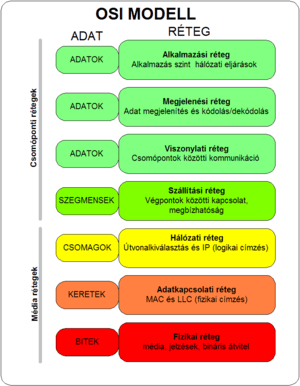
\includegraphics[width=67mm, keepaspectratio]{figures/osi_modell.png}
	\caption{Az OSI modell}
	\label {fig:osi_modell}
\end{figure}
%----------------------------------------------------------------------------

Egy alhálózat egy logikai szegmens egy adott hálózaton belül. Az ilyen szegmenseket
különféle okokból hoznak létre, ideértve elsősorban az adminisztratív és biztonsági
szempontokat. A hálózati adminisztrátor egy készlet szabályt alkalmazhat egy
alhálózatra, míg más szabályokat választhat egy másikra. A routerek képesek
összekapcsolni az alhálózatokat, így a hosztok csomagokat cserélhetnek az
alhálózati határok átlépése nélkül. Egy routernek megfelelően konfigurálva kell
lennie a hálózati útvonalak létrehozásához ezek között az alhálózatok között.
Ezzel szemben egy tipikus kapcsoló nem képes összekapcsolni az alhálózatokat.
Egy virtuális LAN (VLAN) egy másik módszer a hálózat szegmentálására. 
Szemben az alhálózatokkal, ez egy biztonságosabb módja a hosztok elkülönítésére egymástól.

%----------------------------------------------------------------------------
\subsection{Hálózati topológiák}
%----------------------------------------------------------------------------
A csomópontok különböző módon kapcsolódhatnak össze. A topológia meghatározása
az egyik legfontosabb döntés, amelyet egy hálózat tervezésekor hozni kell. A
csillag topológia sok szempontból a preferált megoldás. Több hoszt egy
útválasztó eszközhöz, például egy kapcsolóhoz vagy routerhez csatlakozik. A mai
hálózatok gyakran két csillagszintet kombinálnak. Ezt gerinc/levél architektúrának
nevezik. A központi kapcsoló/router (gerinc) általában több forgalmat továbbít,
mint a perifériális kapcsoló (levél), mivel a szegmensek közötti legtöbb
forgalom áthaladhat rajta. Ha a gerinc és a levél közötti nagy sávszélességű
kapcsolat nem képes egyszerre továbbítani az összes hoszt forgalmát, akkor ez a
tervezési forma blokkoló. Az ellentéte egy nem blokkoló hálózattervezés, ahol a
nagy sávszélességű kapcsolatok képesek az összes a hozzájuk csatlakoztatott
hoszt teljes forgalmát továbbítani. A gyűrű topológiának több interfésze is lehet:
legalább kettőre van szükség egy gyűrű topológia megvalósításához. Minden két
csomópont közötti kapcsolat teljes sávszélességet kínál, és a csomópontokra
hárul a feladat, hogy továbbítsák a csomagokat a gyűrűn belül. Ebben az
értelemben mindegyik csomópont úgy működik, mint egy kapcsoló, csomagokat
továbbítva két interfésze között. A gyűrű topológia választása gyakran ésszerű,
amikor nagy távolságokat kell áthidalni, és a kapcsolatok költségesek.
Gyakorlati példák a különböző helyszínek közötti hálózatok, de gyűrűket alkotnak
olyan eszközök csatlakoztatására is, amelyek esetében nincs hely egy további
kapcsoló számára. A gyűrű topológiák beépített redundanciát kínálnak minden
eszközhöz hozzáférhetünk, még akkor is, ha egy kapcsolat elszakad.

%----------------------------------------------------------------------------
\subsection{Unicast és Multicast} %Egyedi és Csoportos Küldés
%----------------------------------------------------------------------------

Amikor egy eszköz csomagot küld egy másik eszköznek, ezt unicast mechanizmusnak
nevezzük. Egy ilyen kapcsolatnak pontosan egy küldője és egy fogadója van. Az
unicast gyakran használja a Transmission Control Protocol (TCP)-t, ahol a fogadó
minden egyes csomag sikerült átvételéről visszaigazolást küld a küldőnek. Ha a
visszaigazolás nem érkezik meg, a küldő automatikusan újraküldi a csomagot. 
Az UDP (User Datagram Protocol) egy alternatíva a TCP-nek. Ebben az esetben a küldő
bízik abban, hogy a csomagok sikeresen megérkeznek a fogadóhoz. Nincs
visszaigazolás, és ha a csomag elveszik, a tartalma is elveszik. Bár ez
váratlan lehet, ez valójában a preferált átviteli mód a szakmai audio hálózatok
számára. Mivel az időkésleltetés alacsonynak kell lennie, nem engedhető meg a
csomagok újraküldése, mert az időt vesz igénybe, és ezzel növelné az általános
időkésleltetést. Az élő audio csomagvesztés esetén a legjobb, ha folytatjuk a
következő audio minták lejátszását, anélkül hogy megpróbálnánk helyreállítani az
előzőt. Az audio alkalmazásokban gyakran szükség van arra, hogy egy audio jelet
több helyre párhuzamosan fogadjanak, például egy mikrofonjel, amelyet
párhuzamosan továbbítanak a front-of-house és a monitoring keverőpultoknak. Akár
egy harmadik hely is létezhet, például egy felvevő eszköz. 
Amikor a küldő unicast módban továbbítja a csomagokat, az audio jel három csomagként
érkezik azonos tartalommal, de különböző címzési címekkel. Ez felesleges
processzor terhelést jelent a küldő eszköz számára, és emellett sávszélességet
foglal el mindhárom célhoz. Ezt lehet optimalizálni a multicast használatával. 
Számos előnye van, ideértve a küldőre nehezedő kevesebb processzor terhelést 
és az általános forgalom csökkenését a hálózaton. 
A küldő multicast címekre címezi a csomagokat, és nem hoszt címekre. Nem tudja, melyik
címzetteknek érkeznek meg a csomagok. A multicast címek hasonlóak a
rádiófrekvenciákhoz: bárki, aki érdeklődik, bekapcsolhatja és fogadhatja a
tartalmat. A küldő csak egyszer helyezi az audio adatokat egy csomagba, elküldi
egy multicast címre, és a vevőknek tudniuk kell, melyik multicast címre akarnak
hallgatni. A multicast címek alapvetően nem kapcsolódnak alhálózatokhoz, mivel nem
kapcsolódnak a csomópontokhoz és az IP-címekhez. Ezért a multicast csomagok
áthaladnak az alhálózatokon, hacsak nincsenek elkülönítve VLAN-okkal. 
Amennyiben a hálózatunk nem kizárólag az audio jelek továbbítására 
készült speciálisan, néhány eszköz lehet a hálózaton, amelyeknek semmi közük az audiohoz.
Ezért fontos, hogy a multicast forgalom csak
azokhoz a hosztokhoz jusson el, amelyek érdeklődnek iránta. Ennek a megoldása az
IGMP snooping (Internet Csoportkezelési Protokoll). 
Az összes tárgyalt audio hálózati technológia alapértelmezetten
támogatja az IGMP snooping-ot. Ha be van kapcsolva a kapcsolóban, akkor a
multicast-csomagok csak azokon az interfészeken kerülnek elküldésre, ahol a
csatlakoztatott hosztoktól időszakos IGMP kérések érkeznek. Ha nincs beérkező
kérés, akkor a megfelelő multicast leáll, így nem jut felesleges forgalom a
kapcsolaton. Az IGMP snoopingot egyfajta zsilippel lehetne összehasonlítani,
amely alapértelmezetten zárva van, és csak kérésre nyílik meg. Erősen ajánlott
az IGMP snooping bekapcsolása egy multicast hálózatban minden kapcsolóban.

%----------------------------------------------------------------------------
\subsection{Eszköz- és Adatfolyam-felfedezés}
%----------------------------------------------------------------------------

Az AES67 audió szabvány nem határozza meg, hogyan fedezhetik fel egymást a
hálózati eszközök, vagy hogy mely adatfolyamok érhetők el a hálózaton.
Az összes ismert technológia a bonjour vagy mDNS mechanizmust használja eszközeik számára
az egymásról való értesítésre. 
Minden eszköz fix és ismert multicast cím (224.0.0.251) felé küld
üzeneteket, amiket más eszközök elérnek, így értesülnek egymás létezéséről a hálózatban.
Ennek a mechanizmusnak egyik korlátja az, hogy nem működik nagy telepítésekben,
ahol több alcímen vagy VLAN-on vannak. Ezen esetekre a gyártók kifejlesztettek
saját megoldásokat (például Audinate a Dante Domain Manager) vagy
követik az audio/video NMOS szabványt a felismeréshez és kapcsolatkezeléshez.
Az audio adatfolyamokat a gyártótól függően két mechanizmus egyikével fedezik fel. Ahogy
az eszközök felfedezésénél, mindkettő előre meghatározott multicast címet
használ az adatfolyam-információk terjesztésére, hogy a címzettek megtalálják az
elérhető adatfolyamokat és azok paramétereit:

%----------------------------------------------------------------------------
\begin{itemize}
	\item Session Announcement Protocol (SAP) - minden Dante termék által használt (Multicast cím: 239.255.255.255)
\end{itemize}

\begin{itemize}
	\item Bonjour / mDNS - minden más technológiában használt (Multicast cím: 224.0.0.251) 
\end{itemize}
%----------------------------------------------------------------------------
Szerencsére a jelenlegi termékek többsége
lehetővé teszi mindkét protokoll egyidejű aktiválását, így egy adott audio
adatfolyam mindkét mechanizmuson keresztül párhuzamosan bejelenthető.

%----------------------------------------------------------------------------
\subsection{Redundancia}
%----------------------------------------------------------------------------
Az audiohálózatok kezdeti napjaiban egyes felhasználók kételkedtek az IT
hardverek megbízhatóságában. Annak ellenére, hogy a széles körben elterjedt
IT-berendezések jól beváltak és gyakran megbízhatóbbak, mint a hagyományos
audioberendezések. Emellett a legtöbb IT-hálózati komponens több diagnosztikai
mechanizmust kínál a berendezések hibájának gyors felismeréséhez és megoldásához.
%----------------------------------------------------------------------------
\subsubsection{Spanning Tree Protocol (STP)}
%----------------------------------------------------------------------------
Ha a kapcsolókat úgy kötik össze, hogy hurok jön létre, fennáll annak a veszélye, 
hogy a csomagok végtelenül áramlanak a hurokban. 
Ezt az `visszacsatoló hurok' jelenséget a hálózati hardver automatikusan észleli az
STP segítségével, és ha hurokra bukkan, a kapcsoló automatikusan kikapcsol egyik
kapcsolatot. Az STP-t továbbá felhasználhatják a rendszer véletlen
kapcsolatvesztések elleni védelmére is, beleértve a kábelvágásokat is. 

Abból a  megközelítésből áll, hogy szándékosan létrehoznak hurkokat, majd a rendszer
inaktiválja az egyiket. Ha valamelyik kábel véletlenül kiesik, a rendszer
másodperceken belül észleli ezt, és újraaktiválja a passzív kapcsolatot. Ebben
az időszakban az audio néhány másodpercig megszakad, de még mindig sokkal
gyorsabb, mint a manuális hibakeresés és az új kábel telepítése. 
A legtöbb rendszerben az STP alapértelmezetten engedélyezve van. 
%----------------------------------------------------------------------------
\subsubsection{Link Aggregáció}
%----------------------------------------------------------------------------
Ha egy adott kapcsolat különösen fontos egy telepítésben, két vagy több kábelt párhuzamosan
lehet csatlakoztatni a biztonság érdekében. 
Bár az ilyen link aggregáció fő célja két kapcsoló közötti sávszélesség növelése, 
ez is költséghatékony módszer lehet egy kapcsolat véletlen leválasztásának
vagy kábelvágásának biztosítására. Tipikus eset például egy színpad, amely egy keverőhöz
csatlakozik. A kapcsolóknak mindkét végén ugyanúgy kell konfigurálni: két vagy
több interfészt kell kijelölni Link Aggregációs Csoportként, és azok
egyetlen interfészként jelennek meg a kapcsolón. Gyakorlatban a linkaggregáció
alkalmazása a kábelproblémák csökkentése érdekében nagyon hasznos lehet
egyszerűsége miatt, hiszen a felhasználónak csak egy további kábelt kell
biztosítania, és azonosítania kell a kapcsolók konfigurációját mindkét végén.
Ugyanakkor a kábelt lekapcsoláskor előfordulhat, hogy az audioátvitel
néhány másodpercig megszakad, mielőtt a kapcsoló alternatív kapcsolatot
aktiválna.
%----------------------------------------------------------------------------
\subsubsection{ Adatfolyam redundancia}
%----------------------------------------------------------------------------
A legbiztonságosabb de egyben legdrágább módja a redundancia megvalósításának
egy hálózatban az, ha két különálló audiohálózatot hoznak létre, 
két független utat biztosítva a küldő és a fogadó között. 
Ebben a felállásban minden csomópontnak két hálózati interfészt
kell biztosítania. A küldő két azonos audio tartalommal rendelkező csomagot hoz létre,
mindkettőre azonos PTP-időbélyegzőt nyom, majd elküldi mindkét hálózaton.
A fogadó végén mindkét csomagot fogadják és kicsomagolják. Még akkor is, ha az egyik csomag
elveszik, a megmaradt csomag tartalmazza az összes információt, és biztosítja,
hogy az audio zavartalanul folytatódik. Valójában ez a mechanizmus az egyetlen
megközelítés egy hálózatban a véletlenszerű csomagvesztés kompenzálására anélkül,
hogy meg kellene ismételni azokat a küldőtől és ezzel késleltetést hozzáadva a rendszerhez.
%----------------------------------------------------------------------------
\section{AES67}
%----------------------------------------------------------------------------
Az AES67 szabvány szerint az összes eszköznek meg kell felelnie az
alábbi minimális specifikációknak: 

%----------------------------------------------------------------------------
\begin{itemize}
	\item Unicast és multicast támogatása
	\item UDP/RTP protokollok használata
	\item DSCP címkék beállítása meghatározott értékekre,QoS támogatás 
	\item Nincs meghatározott automatikus eszköz- és adatfolyam-felfedezés 
	\item PTPv2 szabvány használata az időszinkronizációhoz
	\item PTP profil Standard (a gyakorlatban a Dante jelenleg magasabb szinkronizációs rátát igényel)
	\item Küldőknek ki kell adniuk egy SDP fájlt
	\item A fogadóknak érteniük kell egy SDP fájlt
	\item A fogadó puffernek legalább 3 ms hangot kell tudnia tárolni
	\item Adatfolyam formátumok
	\item Egytől nyolc csatorna (a küldő választhat egy fix számot, de a fogadóknak képesnek kell lenniük rugalmasan fogadni bármelyik lehetőséget).
	\item 24 bites és 16 bites felbontás (a küldő választhat egyet, de a fogadóknak mindkettőt érteniük kell) 
	\item 48 kHz mintavételi frekvencia 1 ms csomagidő (48 minta)
	\item A multicast címek 239.0.0.0 és 239.255.255.255 között vannak 
\end{itemize}


A szabványban sok további paraméter és érték szerepel, de ezek nem szerepelnek a
fent felsorolt minimális követelmények között.

%----------------------------------------------------------------------------
\section{Audinate Dante}
%----------------------------------------------------------------------------
\subsection{A Dante hálózatok áttekintése}
%----------------------------------------------------------------------------
A 2021-es Covid-19 járvány alatt lehetőségem volt egy széleskörű átfogó Dante
kurzusra beiratkozni, amelyet a Dante gyártója, az Audinate szervezett. A kurzus
egy átfogó mély áttekintést nyújtott a Dante hálózatokról. Ebben a fejezetben
a fő forrásomnak a belsős oktatóanyagot fogom használni, amelyet a kurzus
során kaptam, pontos és részletes információkat nyújtva a Dante hálózatokról.
Ez a dokumentum csak azok számára elérhető, akik részt vettek a kurzuson.
A Dante hanghálózatok digitális hanghálózati technológiát képviselnek, amely
lehetővé teszi a hang elosztását és útválasztását a szabványos Ethernet
hálózatokon keresztül. Az ausztrál Audinate vállalat fejlesztette ki a Dante-t,
amely a szabványos Internet Protocol (IP) hálózatokat használja a magas minőségű,
alacsony késleltetésű hangátvitelhez eszközök között. Ez lehetővé tesz
nagyobb rugalmasságot és skálázhatóságot a hagyományos analóg hangrendszerekhez
képest, valamint biztosítja a hangrendszer integrálását egy meglévő IT infrastruktúrába.
A Dante hanghálózatokat széles körben alkalmazzák, ideértve a koncerthangosítást,
rádiózást, stúdiófelvételeket, vállalati és konferenciaközpontokat, és még sok mást.
A technológia támogat számos hangformátumot és mintavételi rátát, és lehetővé
teszi akár több száz hangcsatorna egyidejű átvitelét egyetlen hálózaton keresztül.
Emellett a Dante hanghálózatok távolról is vezérelhetők és monitorozhatók,
megkönnyítve a nagy, összetett hangrendszerek beállítását és kezelését.
%----------------------------------------------------------------------------
\begin{figure}[H]
	\centering
	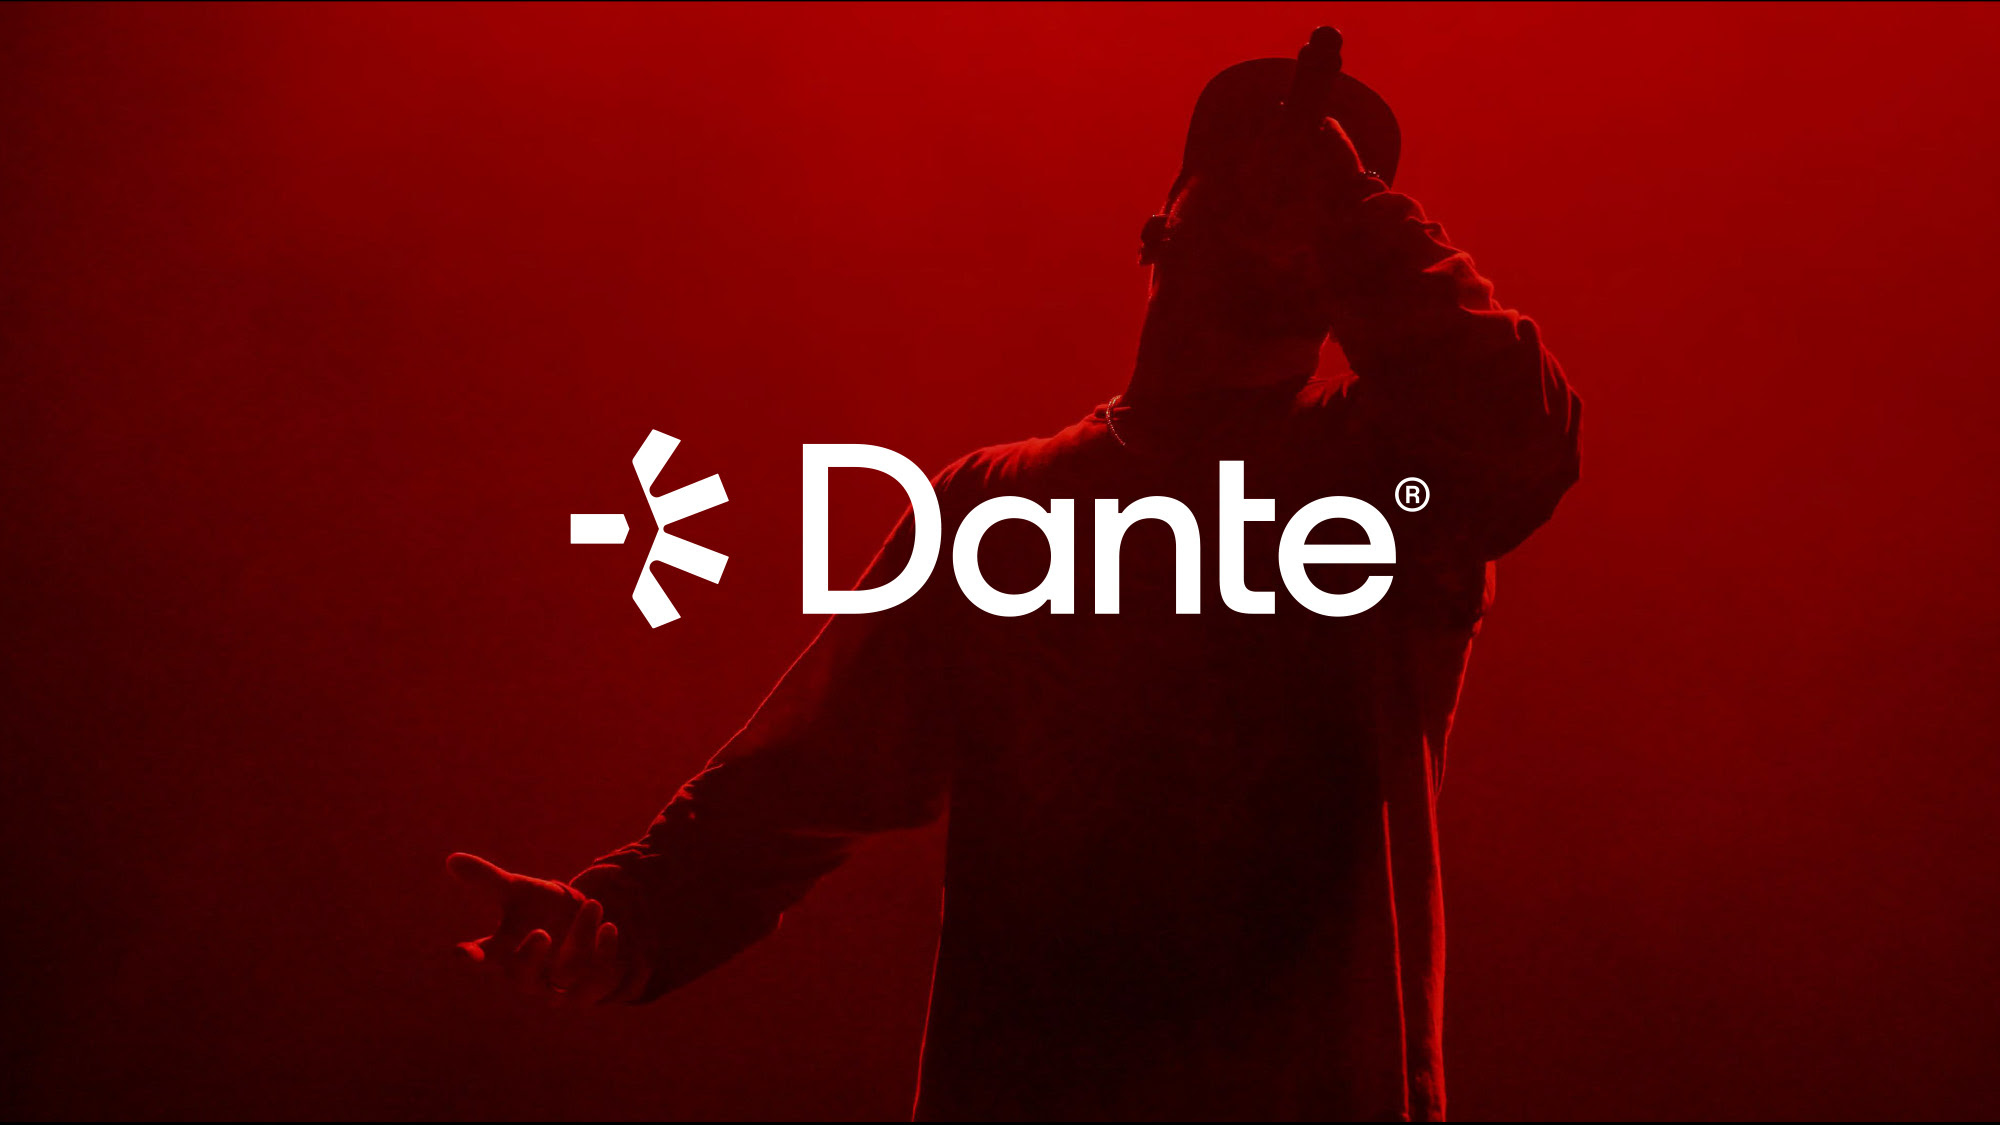
\includegraphics[width=200px, keepaspectratio]{figures/dante_visual.jpg}
	\caption{Audinate Dante fantázia ábra}
	\label {fig:dante_visual}
\end{figure}
%----------------------------------------------------------------------------
\subsubsection{Több mintavételi ráta és bitmélység}
%----------------------------------------------------------------------------
A rendszer képes egyidejűleg több bitmélységet kezelni. Ennek informatikai háttere a
a következő képpen néz ki. Ha egy 32 bites hangforrásunk van, de a másik eszköz
csak 24 bites hangot tud fogadni, akkor a Dante a 32 bites hangot 24 bitesre tudja 
alakítani.

%----------------------------------------------------------------------------
\begin{align*}
	\begin{array}{|c|c|}
	\hline
	\text{Hangminták} & \text{Bitmélység} \\
	\hline
	\text{11110000 11110000 11110000 11110000} & \text{32 bites} \\
	\hline
	\text{11110000 11110000 11110000} & \text{24 bites} \\
	\hline
	\end{array}
\end{align*}
%----------------------------------------------------------------------------
	
Amint a példában látszik, 32 bites hangból úgy kaptunk 24 bites hangot, 
hogy egyszerűen csak elhagytuk az utolsó 8 bitet. Ez a folyamat visszafelé is működik,
ha 24 bites hangot kell 32 bites hanggá alakítani, akkor az utolsó 8 bitet 0-val kell feltölteni.

%----------------------------------------------------------------------------	
\begin{align*}
	\begin{array}{|c|c|}
	\hline
	\text{Hangminták} & \text{Bitmélység} \\
	\hline
	\text{11110000 11110000 11110000} & \text{24 bites} \\
	\hline
	\text{11110000 11110000 11110000 00000000} & \text{32 bites} \\
	\hline
	\end{array}
\end{align*}
%----------------------------------------------------------------------------

Mintavételezési frekvencia eltérést csak abban az esetben tudja kezelni, ha a
bitmélység is eltérő. Amennyiben a bitmélység azonos, de a mintavételezési
frekvencia eltérő, akkor a rendszer nem képes a hangot továbbítani.
Ez a mechanizmus egy egyszerű mechanikai példával jól megérhető és leírható.
Tegyük fel van két fogaskerekünk. Amennyiben a mintavételezési frekvencia azonos, és a 
bitmélység eltérő, akkor a fogaskerekek egymásba illeszthetőek és csak a fogaskerekek
mélysége fog eltérni. Amennyiben a mintavételezési frekvencia eltérő, akkor a fogaskerekek
nem illeszthetőek egymásba, és nem tudjuk továbbítani a hangot. Ebben az esetben már egy
konverterre lesz szükségünk, amely képes a két fogaskereket összeilleszteni számunkra.
Egy fontos kitétel van ahhoz, hogy a több mintavételi ráta egyszerre megfelelően működjön,
az pedig az egységes órajel az összes mintavételi frekvenciához.


%----------------------------------------------------------------------------
\subsubsection{Hálózati topológiák}
%----------------------------------------------------------------------------
A Dante rendszerek alapvetően kétféle módban tudnak üzemelni. Az első a
switched (kapcsolt) mód, amelyben az eszközökön található két Ethernet port
egy hálózatot alkot. Ebben a módban tudunk Daisy Chain (füzéres) topológiát kialakítani,
amelyben az egyik eszköz a másikhoz csatlakozik, és így tovább. Továbbá csillagtopológiát
is kialakíthatunk, amelyben minden eszköz egy központi kapcsolóhoz csatlakozik.
%----------------------------------------------------------------------------
\begin{figure}[H]
	\begin{minipage}{0.5\textwidth}
		\centering
		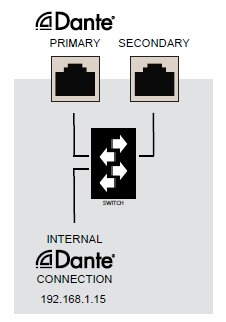
\includegraphics[width=100px, keepaspectratio]{figures/dante-switched-mode.jpg}
		\caption{Kapcsolt mód}
		\label{fig:dante_switched}
	\end{minipage}%
	\begin{minipage}{0.5\textwidth}
		\centering
		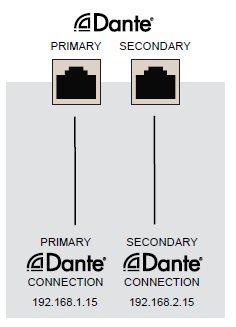
\includegraphics[width=100px, keepaspectratio]{figures/dante-redundant-mode.jpg}
		\caption{Redundáns mód}
		\label{fig:dante_redundant}
	\end{minipage}
\end{figure}

%----------------------------------------------------------------------------
A másik mód a redundant (redundáns) mód, amelyben az eszközökön található két
Ethernet port két különálló hálózatot alkot. Ebben a módban a hálózat redundáns
kialakítású, és a hálózat egyik része automatikusan átveszi a másik rész szerepét,
ha az meghibásodik.
Néhány Dante eszköznek létezik egy harmadik Ethernet portja, amelyet konfigurálási
és vezérlési célokra használnak.
%----------------------------------------------------------------------------
\subsubsection{Késleltetés}
%----------------------------------------------------------------------------
A késleltetés az az idő, amely szükséges a folyamat végrehajtásához. Például
az idő amíg a bemeneti oldalon egy hangjel feldolgozásra kerül, és a kimeneti
oldalon megjelenik. 
Két fő mértékegységet használunk a késleltetés mérésére:
%----------------------------------------------------------------------------
\begin{equation}
	\label{eq:milliseconds}
	1 \text{ másodperc} = 1000 \text{ milli másodperc}, \quad \text{azaz} \quad 1 \text{ ms} = 0.001 \text{ s}
\end{equation}
%----------------------------------------------------------------------------
%----------------------------------------------------------------------------
\begin{equation}
	\label{eq:microseconds}
	1 \text{ másodperc} = 1000000 \text{ mikro másodperc}, \quad \text{azaz} \quad 1 \mu\text{s} = 0.000001 \text{ s}
\end{equation}
%----------------------------------------------------------------------------
A Dante eszközök lehetővé teszik a késleltetés teljesítményének meghatározását. 
A 0.1 milliszekundumos késleltetés az a késleltetés, amely már kapcsoló lépés biztos.
Ha két eszköz különböző késleltetésű, akkor a nagyobb érték lesz az irányadó.
Egy megfelelően konfigurált modern Dante hálózatban a késleltetés 1 ms körüli értéket vesz fel.
Ez azt is jelenti, hogy például egy dobos előbb hallja a hangszerét a fülmonitoron, mint a saját dobját.






%----------------------------------------------------------------------------
\subsection{Összehasonlítás a hagyományos hangrendszerekkel}
%----------------------------------------------------------------------------
A hagyományos hangrendszerek általában analóg kábelekre és csatlakozókra
támaszkodnak a hangjelek eszközök közötti átviteléhez. Ezek a rendszerek
korlátozottak lehetnek rugalmasságban, skálázhatóságban és az egyidejűleg
átvihető hangcsatornák számában. Emellett hajlamosak bonyolultabbá válni a
beállítás és kezelés szempontjából, mivel minden hangcsatornához külön kábel és
csatlakozás szükséges. A Dante hanghálózatok jóval több hangcsatornát is támogatnak,
mint a hagyományos analóg rendszerek, és távolról is vezérelhetők és
monitorozhatók, lehetővé téve a nagy, összetett hangrendszerek könnyű
beállítását és kezelését. A Dante hanghálózatok további előnye, hogy képesek
hangot továbbítani hosszú távolságokon anélkül, hogy a minőség romlana. A
hagyományos analóg rendszerek zajra és jelveszteségre hajlamosak hosszú kábelek
esetén, míg a digitális hangjelek, amelyeket az Ethernet hálózatokon
továbbítanak, minimális minőségveszteséggel juthatnak el nagy távolságokra.
%----------------------------------------------------------------------------
\begin{table}[htbp]
    \centering
    \caption{Digital Snake és DigitalAVNetwork Jelút opciók}
    \begin{tabular}{@{}lll@{}}
        \toprule
        \textbf{Kérdés} & \textbf{Pont-pont között} & \textbf{Hálózati megoldás} \\ \midrule
        Hová megy a jel? & Lineáris kábelút & Bárhol a hálózaton \\
        Hogyan változtassuk meg a jelútvonalat? & Mozgassuk a kábelt & Egy egérkattintással \\
        Szétválaszthatjuk-e a jeleket? & Nem & Igen - a hálózaton \\
        Megosztható-e a kábel más jelekkel? & Nem & Igen - közös infrastruktúra \\
        \bottomrule
    \end{tabular}
    \label{tab:digital-snake-vs-digitalavnetwork-hu}
\end{table}
%----------------------------------------------------------------------------
\begin{figure}[H]
	\centering
	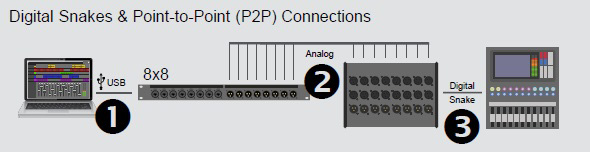
\includegraphics[width=\linewidth, keepaspectratio]{figures/dsnake-p2p.jpg}
	\caption{Digital Snake és Pont-pont közötti (P2P) kapcsolatok}
	\label {fig:dsnake-p2p}
\end{figure}
%----------------------------------------------------------------------------
\begin{figure}[H]
	\centering
	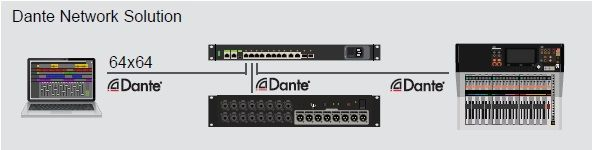
\includegraphics[width=\linewidth, keepaspectratio]{figures/dante-solution.jpg}
	\caption{Dante hálózati megoldás}
	\label {fig:dante-solution}
\end{figure}
%----------------------------------------------------------------------------




%----------------------------------------------------------------------------
\subsection{Dante hálózatok technikai részletei}
%----------------------------------------------------------------------------
A Dante hanghálózatok két fő komponensből állnak: Dante eszközökből
és Dante hálózatokból. A Dante eszközök olyan hangeszközök, amelyeket
kifejezetten a Dante protokollhoz terveztek, mint például hangkártyák, erősítők
és hangszórók. Ezeket az eszközöket szabványos Ethernet kábelekkel és
kapcsolókkal lehet csatlakoztatni a Dante hálózathoz.
A hálózatot az Audinate Dante Controller szoftverrel lehet
konfigurálni, amely lehetővé teszi a hang elosztását és útválasztását az
eszközök között. A szoftver továbbá lehetővé teszi az eszközök távoli vezérlését
és monitorozását a hálózaton. Ezek a hanghálózatok támogatnak számos
hangformátumot és mintavételi rátát, és képesek egyszerre több száz hangcsatorna
átvitelére egyetlen hálózaton keresztül. A technológia továbbá támogat olyan
fejlett funkciókat, mint a Dante Domain Manager (DDM) a biztonságos
hangátvitelhez, valamint a Dante Virtual Soundcard (DVS) a számítógépes alapú
hanglejátszáshoz és felvételhez. A Dante hanghálózatok Quality of Service (QoS)
támogatást is nyújtanak, hogy biztosítsák, hogy a hangátvitel elsőbbséget
élvezzen más hálózati forgalommal szemben. Ez segít minimalizálni a hálózati
torlódás lehetőségét és biztosítani, hogy a hangátvitel minimális késleltetéssel
és magas minőségben történjen.
%----------------------------------------------------------------------------
\subsection{Rugalmasság és skálázhatóság}
%----------------------------------------------------------------------------
A rugalmasság és a skálázhatóság két kulcsfontosságú előnye a Dante
hanghálózatoknak a hagyományos analóg hangrendszerekkel szemben.
Képesek alkalmazkodni különböző hangkonfigurációkhoz és követelményekhez. 
Könnyű eszközöket hozzáadni vagy eltávolítani, megváltoztatni a hangjelek útvonalát, és a rendszert újra
konfigurálni szükség esetén. Ez lehetővé teszi testreszabott audio-megoldások
létrehozását, amelyeket az adott alkalmazás vagy környezet speciális igényeihez
lehet igazítani. 


%----------------------------------------------------------------------------
\subsection{Chipek}
%----------------------------------------------------------------------------
%----------------------------------------------------------------------------
\begin{itemize}
    \item 
    \begin{minipage}[t]{.2\textwidth}
        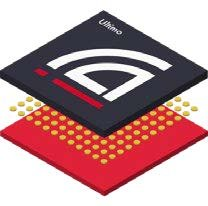
\includegraphics[width=50px,height=50px,keepaspectratio]{figures/ultimo-x.jpg}
    \end{minipage}%
    \begin{minipage}[t]{.8\textwidth}
        \textbf{Dante Ultimo-X - 0x4, 2x2, 4x0}
    \end{minipage}

    \item 
    \begin{minipage}[t]{.2\textwidth}
        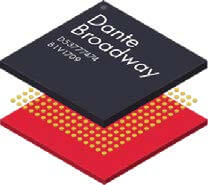
\includegraphics[width=50px,height=50px,keepaspectratio]{figures/broadway.jpg}
    \end{minipage}%
    \begin{minipage}[t]{.8\textwidth}
        \textbf{Dante Broadway - 16x16}
    \end{minipage}

    \item 
    \begin{minipage}[t]{.2\textwidth}
        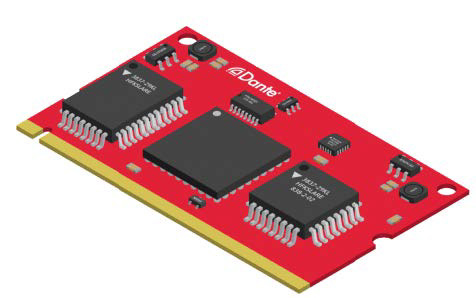
\includegraphics[width=50px,height=50px,keepaspectratio]{figures/brooklyn-ii.jpg}
    \end{minipage}%
    \begin{minipage}[t]{.8\textwidth}
        \textbf{Dante Brooklyn II - 64x64}
    \end{minipage}

    \item 
    \begin{minipage}[t]{.2\textwidth}
        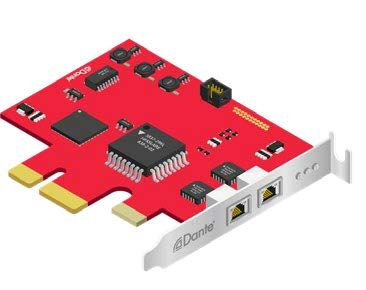
\includegraphics[width=50px,height=50px,keepaspectratio]{figures/pcie-r.jpg}
    \end{minipage}%
    \begin{minipage}[t]{.8\textwidth}
        \textbf{Dante PCIe-R - 128x128}
    \end{minipage}

    \item 
    \begin{minipage}[t]{.2\textwidth}
        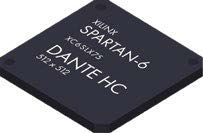
\includegraphics[width=50px,height=50px,keepaspectratio]{figures/dante-hc.jpg}
    \end{minipage}%
    \begin{minipage}[t]{.8\textwidth}
        \textbf{Dante HC (High Capacity) - 512x512}
    \end{minipage}

    \item 
    \begin{minipage}[t]{.2\textwidth}
        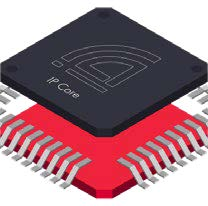
\includegraphics[width=50px,height=50px,keepaspectratio]{figures/shared-processor.jpg}
    \end{minipage}%
    \begin{minipage}[t]{.8\textwidth}
        \textbf{Dante Shared Processor - IP Core 512x512 FPGA and Dante Embedded Platform 64x64 X86/ARM}
    \end{minipage}

    \item 
    \begin{minipage}[t]{.2\textwidth}
        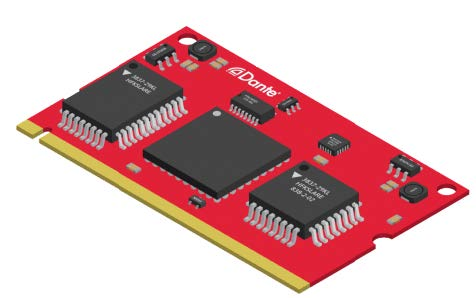
\includegraphics[width=50px,height=50px,keepaspectratio]{figures/dante-av.jpg}
    \end{minipage}%
    \begin{minipage}[t]{.8\textwidth}
        \textbf{Dante AV - V:1, A:8}
    \end{minipage}
\end{itemize}









